\section{Cipher Specifications}

\begin{frame}{A Linear Transformation $\theta$}
  \begin{beamerboxesrounded}{A Linear Transformation ($\theta$)}
    $\theta$ is a linear operation.
    $$
      \theta: b=\theta(a) \Leftrightarrow b_{i, j}=c_{j} a_{i, 0} \oplus c_{j-1} a_{i, 1} \oplus c_{j-2} a_{i, 2} \oplus c_{j-3} a_{i, 3}
    $$
    Here, $c$ is a 1D array and equivalent to below matrix:

    \begin{equation*}
      c   \equiv \begin{bmatrix}
        2 & 1 & 1 & 3 \\
        3 & 2 & 1 & 1 \\
        1 & 3 & 2 & 1 \\
        1 & 1 & 3 & 2
      \end{bmatrix}
    \end{equation*}
  \end{beamerboxesrounded}
\end{frame}

\begin{frame}{A Nonlinear Transformation $\gamma$}
  \begin{beamerboxesrounded}{A Nonlinear Transformation ($\gamma$)}
    $\gamma$ is a nonlinear byte substitution, identical for all bytes.
    $$
      \gamma: b=\gamma(a) \Leftrightarrow b_{i, j}=\mathrm{S}_{\gamma}\left(a_{i, j}\right)
    $$
    Here, $\mathrm{S}$ -box is an invertible 8-bit substitution table.
  \end{beamerboxesrounded}
\end{frame}

\begin{frame}{A Byte Permutation $\pi$}
  \begin{beamerboxesrounded}{A Byte Permutation ($\pi$)}
    $\pi$ is a linear operation. It transposes a matrix.
    $$
      \pi: b=\pi(a) \Leftrightarrow b_{i, j}=a_{j, i}
    $$
    $\pi$ is an involution $\iff$ $\pi^{-1}=\pi$
  \end{beamerboxesrounded}
\end{frame}

\begin{frame}{Bitwise Round Key Addition $\sigma$}
  \begin{beamerboxesrounded}{Bitwise Round Key Addition ($\sigma$)}
    $\sigma$ is a linear opeartion.

    $$
      \sigma\left[k^{t}\right]: b=\sigma\left[k^{t}\right](a) \Leftrightarrow b=a \oplus k^{t}
    $$
    $\sigma$ is an involution also hence,
    the inverse of $\sigma\left[k^{t}\right]$ is $\sigma\left[k^{t}\right]$ itself.
  \end{beamerboxesrounded}
\end{frame}

\begin{frame}{Key scheduling}
  \begin{beamerboxesrounded}{The Round Key Evolution ($\psi$)}
    The round keys $k^{t}$ are derived from the cipher key $K$. $k^{0}$ equals the cipher key $K$.$\psi$ is a affine transfomation.
    $$
      \psi: k^{t}=\psi\left(k^{t-1}\right)
    $$
  \end{beamerboxesrounded}
\end{frame}

\begin{frame}{Rounds}
  \begin{beamerboxesrounded}{Rounds}
    There are total eight rounds in SQUARE Cipher proceeded by a key addition $\sigma\left[k^{0}\right]$ and by $\theta^{-1}$.

    Every round is denoted by $\rho\left[k^{t}\right]$.
    $$
      \rho\left[k^{t}\right]=\sigma\left[k^{t}\right] \circ \pi \circ \gamma \circ \theta
    $$

    In first round $\theta^{-1}$ before $\sigma\left[k^{0}\right]$ are also incorporated:-\\
    hence,
    $$
      \begin{aligned}
        \rho\left[k^{1}\right] \circ \sigma\left[k^{0}\right] \circ \theta^{-1}                               \\ &=\sigma\left[k^{1}\right] \circ \pi \circ \gamma \circ \theta \circ \sigma\left[k^{0}\right] \circ \theta^{-1} \\
         & =\sigma\left[k^{1}\right] \circ \pi \circ \gamma \circ \sigma\left[\theta\left(k^{0}\right)\right]
      \end{aligned}
    $$
  \end{beamerboxesrounded}
\end{frame}

\begin{frame}{Rounds}
  All eight rounds of SQUARE Cipher:

  \begin{beamerboxesrounded}{SQUARE}
    \begin{flalign*}
      SQUARE[k]&=\rho\left[k^{8}\right] \circ \rho\left[k^{7}\right] \circ \rho\left[k^{6}\right] \circ \rho\left[k^{5}\right] \circ \rho\left[k^{4}\right] \circ \rho\left[k^{3}\right] \circ \\& \rho\left[k^{2}\right] \circ \rho\left[k^{1}\right] \circ \sigma\left[k^{0}\right] \circ \theta^{-1}
    \end{flalign*}
  \end{beamerboxesrounded}
\end{frame}

\begin{frame}{SQUARE Cipher}
  \begin{figure}
    \centering
    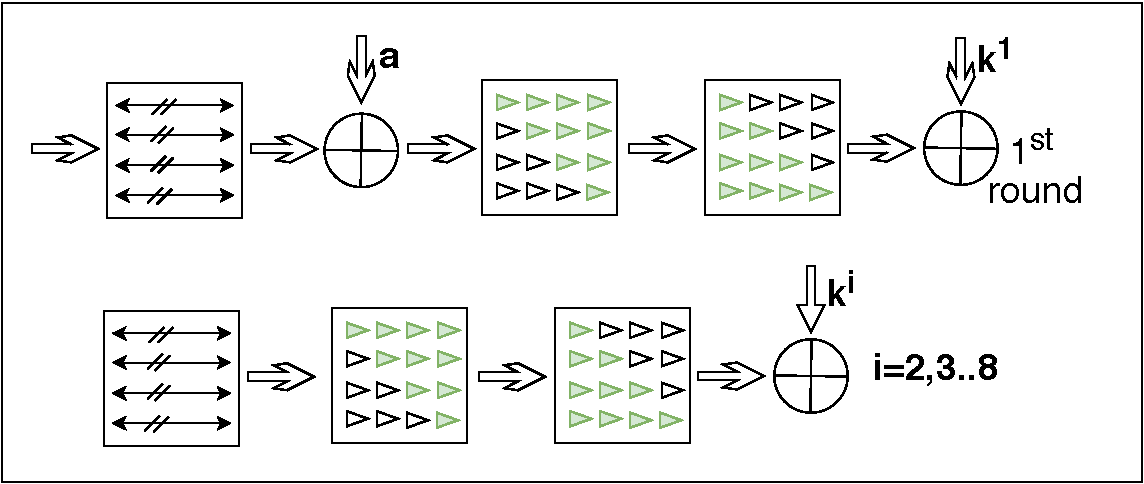
\includegraphics[width=\linewidth]{Square_cipher_diagram}
    \caption{SQUARE cipher encryption}
  \end{figure}
\end{frame}
\begin{frame}{Properties}
  \begin{itemize}
    \item {Inverse Cipher}
          Square has been designed in such a way that the structure of its inverse is equal to that of the cipher itself, with the exception of the key schedule.
          \begin{flalign*}
            \text { SQUARE }^{-1}[k]&=
            \qquad  \theta \circ \sigma\left[k^{0}\right] \circ \rho^{-1}\left[k^{1}\right] \circ \rho^{-1}\left[k^{2}\right] \\&  \circ \rho^{-1}\left[k^{3}\right] \circ              \rho^{-1}\left[k^{4}\right] \circ \rho^{-1}\left[k^{5}\right] \circ \rho^{-1}\left[k^{6}\right] \\&  \circ \rho^{-1}\left[k^{7}\right] \circ \rho^{-1}\left[k^{8}\right]
          \end{flalign*}

          Round transformation  of Inverse cipher as:-
          $$
            \rho^{\prime}\left[k^{t}\right]=\sigma\left[k^{t}\right] \circ \pi \circ \gamma^{-1} \circ \theta^{-1}
          $$
          Above expression shows the same structure of $\rho{prime}$ as $\rho$ itself, except that $\gamma$ and $\theta$ are replaced by $\gamma^{-1}$ and $\theta^{-1}$    respectively.
  \end{itemize}
\end{frame}

\begin{frame}{Properties}
  \begin{itemize}
    \item {Confusion\\}
          Nonlinear Transformation $\gamma$ adds confusion property in the cipher.
    \item{Diffusion\\}
          In Square Cipher, transformation operations (Linear Transformation $\theta$, Byte Permutation $\pi$ add diffusion property in the cipher.
    \item{Security margin\\}
          Like AES in SQUARE we also have safety rounds. Integral attack was known up to six rounds so to make it secure cipher was extended up to eight rounds. Now, there are total eight rounds so last two rounds are for security purpose of cipher.
  \end{itemize}
\end{frame}
% \end{document}
